\begin{center}
\textbf{Emile\ Durkheim}\\
	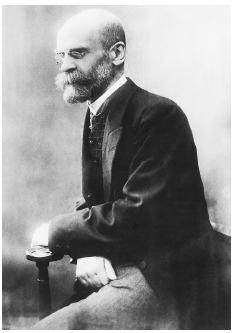
\includegraphics[scale=0.5]{images/durkheim}\\
	 \emph{(Épinal, Francia, 15 de abril 1858 — París, Francia, 15 de noviembre 1917)}\\
\end{center}
Uno de los fundadores de la sociología moderna, junto a Max Weber y Karl Marx.
Fundador de la primera revista dedicada a las ciencias sociales, el \emph{Année Sociologique},
con el cual también se identifica al grupo de estudiosos que desarrolló su programa de investigación sociológica.\\

Nació en Épinal, Francia, el 15 de abril 1858 en la región de Lorena.
A pesar de ser hijo de una familia profundamente religiosa (era hijo de un rabino),Durkheim tuvo una vida completamente secular.

Desde joven se sintió atraído por el método científico, que se oponía a su educación basada en la religión.

En muchos de sus trabajos, de hecho, estuvo dedicado a demostrar que los fenómenos religiosos provienen de factores sociales más que divinos.

Sus antecedentes judíos, sin embargo, moldearon su sociología, y muchos de sus estudiantes y colaboradores fueron compañeros judíos o parientes de sangre.

Durkheim entró a la École Normale Supérieure (Escuela Normal Superior), en 1879.
Su generación fue una de las más brillantes del siglo XIX y muchos de sus compañeros de clase, tales como Jean Jaurès y Henri Bergson se convertirían en importantes figuras de la vida intelectual francesa.

En la ENS (Escuela Normal Superior), Durkheim estudió con Fustel de Coulanges de su generación cuando se graduó en filosofía en 1882.
En 1887, es nombrado profesor de pedagogía y ciencia social de la Universidad de Burdeos.
Comienza con sus enseñanzas en sociología y fue el primero en enseñar esta ciencia en Francia.
Como consecuencia de los pesares que le causó la muerte de su único hijo, murió en París el 15 de noviembre de 1917.


\newpage
